% Options for packages loaded elsewhere
\PassOptionsToPackage{unicode}{hyperref}
\PassOptionsToPackage{hyphens}{url}
%
\documentclass[
  10pt,
  ignorenonframetext,
]{beamer}
\title{《生物实验设计》\\
第一章\(~\)资料整理与特征数计算}
\author{王超\\
\strut \\
广东药科大学\\
Email:
\href{mailto:wangchao@gdpu.edu.cn}{\nolinkurl{wangchao@gdpu.edu.cn}}}
\date{2022-07-25}

\usepackage{pgfpages}
\setbeamertemplate{caption}[numbered]
\setbeamertemplate{caption label separator}{: }
\setbeamercolor{caption name}{fg=normal text.fg}
\beamertemplatenavigationsymbolsempty
% Prevent slide breaks in the middle of a paragraph
\widowpenalties 1 10000
\raggedbottom
\setbeamertemplate{part page}{
  \centering
  \begin{beamercolorbox}[sep=16pt,center]{part title}
    \usebeamerfont{part title}\insertpart\par
  \end{beamercolorbox}
}
\setbeamertemplate{section page}{
  \centering
  \begin{beamercolorbox}[sep=12pt,center]{part title}
    \usebeamerfont{section title}\insertsection\par
  \end{beamercolorbox}
}
\setbeamertemplate{subsection page}{
  \centering
  \begin{beamercolorbox}[sep=8pt,center]{part title}
    \usebeamerfont{subsection title}\insertsubsection\par
  \end{beamercolorbox}
}
\AtBeginPart{
  \frame{\partpage}
}
\AtBeginSection{
  \ifbibliography
  \else
    \frame{\sectionpage}
  \fi
}
\AtBeginSubsection{
  \frame{\subsectionpage}
}
\usepackage{amsmath,amssymb}
\usepackage{lmodern}
\usepackage{iftex}
\ifPDFTeX
  \usepackage[T1]{fontenc}
  \usepackage[utf8]{inputenc}
  \usepackage{textcomp} % provide euro and other symbols
\else % if luatex or xetex
  \usepackage{unicode-math}
  \defaultfontfeatures{Scale=MatchLowercase}
  \defaultfontfeatures[\rmfamily]{Ligatures=TeX,Scale=1}
\fi
% Use upquote if available, for straight quotes in verbatim environments
\IfFileExists{upquote.sty}{\usepackage{upquote}}{}
\IfFileExists{microtype.sty}{% use microtype if available
  \usepackage[]{microtype}
  \UseMicrotypeSet[protrusion]{basicmath} % disable protrusion for tt fonts
}{}
\makeatletter
\@ifundefined{KOMAClassName}{% if non-KOMA class
  \IfFileExists{parskip.sty}{%
    \usepackage{parskip}
  }{% else
    \setlength{\parindent}{0pt}
    \setlength{\parskip}{6pt plus 2pt minus 1pt}}
}{% if KOMA class
  \KOMAoptions{parskip=half}}
\makeatother
\usepackage{xcolor}
\IfFileExists{xurl.sty}{\usepackage{xurl}}{} % add URL line breaks if available
\IfFileExists{bookmark.sty}{\usepackage{bookmark}}{\usepackage{hyperref}}
\hypersetup{
  hidelinks,
  pdfcreator={LaTeX via pandoc}}
\urlstyle{same} % disable monospaced font for URLs
\newif\ifbibliography
\usepackage{color}
\usepackage{fancyvrb}
\newcommand{\VerbBar}{|}
\newcommand{\VERB}{\Verb[commandchars=\\\{\}]}
\DefineVerbatimEnvironment{Highlighting}{Verbatim}{commandchars=\\\{\}}
% Add ',fontsize=\small' for more characters per line
\usepackage{framed}
\definecolor{shadecolor}{RGB}{248,248,248}
\newenvironment{Shaded}{\begin{snugshade}}{\end{snugshade}}
\newcommand{\AlertTok}[1]{\textcolor[rgb]{0.94,0.16,0.16}{#1}}
\newcommand{\AnnotationTok}[1]{\textcolor[rgb]{0.56,0.35,0.01}{\textbf{\textit{#1}}}}
\newcommand{\AttributeTok}[1]{\textcolor[rgb]{0.77,0.63,0.00}{#1}}
\newcommand{\BaseNTok}[1]{\textcolor[rgb]{0.00,0.00,0.81}{#1}}
\newcommand{\BuiltInTok}[1]{#1}
\newcommand{\CharTok}[1]{\textcolor[rgb]{0.31,0.60,0.02}{#1}}
\newcommand{\CommentTok}[1]{\textcolor[rgb]{0.56,0.35,0.01}{\textit{#1}}}
\newcommand{\CommentVarTok}[1]{\textcolor[rgb]{0.56,0.35,0.01}{\textbf{\textit{#1}}}}
\newcommand{\ConstantTok}[1]{\textcolor[rgb]{0.00,0.00,0.00}{#1}}
\newcommand{\ControlFlowTok}[1]{\textcolor[rgb]{0.13,0.29,0.53}{\textbf{#1}}}
\newcommand{\DataTypeTok}[1]{\textcolor[rgb]{0.13,0.29,0.53}{#1}}
\newcommand{\DecValTok}[1]{\textcolor[rgb]{0.00,0.00,0.81}{#1}}
\newcommand{\DocumentationTok}[1]{\textcolor[rgb]{0.56,0.35,0.01}{\textbf{\textit{#1}}}}
\newcommand{\ErrorTok}[1]{\textcolor[rgb]{0.64,0.00,0.00}{\textbf{#1}}}
\newcommand{\ExtensionTok}[1]{#1}
\newcommand{\FloatTok}[1]{\textcolor[rgb]{0.00,0.00,0.81}{#1}}
\newcommand{\FunctionTok}[1]{\textcolor[rgb]{0.00,0.00,0.00}{#1}}
\newcommand{\ImportTok}[1]{#1}
\newcommand{\InformationTok}[1]{\textcolor[rgb]{0.56,0.35,0.01}{\textbf{\textit{#1}}}}
\newcommand{\KeywordTok}[1]{\textcolor[rgb]{0.13,0.29,0.53}{\textbf{#1}}}
\newcommand{\NormalTok}[1]{#1}
\newcommand{\OperatorTok}[1]{\textcolor[rgb]{0.81,0.36,0.00}{\textbf{#1}}}
\newcommand{\OtherTok}[1]{\textcolor[rgb]{0.56,0.35,0.01}{#1}}
\newcommand{\PreprocessorTok}[1]{\textcolor[rgb]{0.56,0.35,0.01}{\textit{#1}}}
\newcommand{\RegionMarkerTok}[1]{#1}
\newcommand{\SpecialCharTok}[1]{\textcolor[rgb]{0.00,0.00,0.00}{#1}}
\newcommand{\SpecialStringTok}[1]{\textcolor[rgb]{0.31,0.60,0.02}{#1}}
\newcommand{\StringTok}[1]{\textcolor[rgb]{0.31,0.60,0.02}{#1}}
\newcommand{\VariableTok}[1]{\textcolor[rgb]{0.00,0.00,0.00}{#1}}
\newcommand{\VerbatimStringTok}[1]{\textcolor[rgb]{0.31,0.60,0.02}{#1}}
\newcommand{\WarningTok}[1]{\textcolor[rgb]{0.56,0.35,0.01}{\textbf{\textit{#1}}}}
\setlength{\emergencystretch}{3em} % prevent overfull lines
\providecommand{\tightlist}{%
  \setlength{\itemsep}{0pt}\setlength{\parskip}{0pt}}
\setcounter{secnumdepth}{-\maxdimen} % remove section numbering
\ifLuaTeX
  \usepackage{selnolig}  % disable illegal ligatures
\fi

\begin{document}
\frame{\titlepage}

\begin{frame}{}
\protect\hypertarget{section}{}
\LARGE 第二章\(~\)资料整理与特征数计算
\end{frame}

\begin{frame}{第一节\(~\)资料的搜集与整理}
\protect\hypertarget{ux7b2cux4e00ux8282ux8d44ux6599ux7684ux641cux96c6ux4e0eux6574ux7406}{}
\end{frame}

\begin{frame}{一、资料的类型}
\protect\hypertarget{ux4e00ux8d44ux6599ux7684ux7c7bux578b}{}
\begin{itemize}
\item
  数量性状资料
\item
  质量性状资料
\end{itemize}
\end{frame}

\begin{frame}{二、资料的搜集}
\protect\hypertarget{ux4e8cux8d44ux6599ux7684ux641cux96c6}{}
\begin{itemize}
\item
  调查
\item
  试验
\end{itemize}
\end{frame}

\begin{frame}{三、资料的整理}
\protect\hypertarget{ux4e09ux8d44ux6599ux7684ux6574ux7406}{}
\begin{itemize}
\item
  原始资料的检查与核对
\item
  频数分布表
\item
  频数分布图
\end{itemize}
\end{frame}

\begin{frame}[fragile]{频数分布表}
\protect\hypertarget{ux9891ux6570ux5206ux5e03ux8868}{}
100只鸡每月产蛋数(用\texttt{rnorm}随机生成这样一组数据)

\begin{Shaded}
\begin{Highlighting}[]
\FunctionTok{set.seed}\NormalTok{(}\DecValTok{2022}\NormalTok{)}
\NormalTok{egg }\OtherTok{\textless{}{-}} \FunctionTok{round}\NormalTok{(}\FunctionTok{rnorm}\NormalTok{(}\DecValTok{100}\NormalTok{, }\AttributeTok{mean =} \DecValTok{14}\NormalTok{, }\AttributeTok{sd =} \FloatTok{1.5}\NormalTok{))}
\NormalTok{egg}
\end{Highlighting}
\end{Shaded}

\begin{verbatim}
##   [1] 15 12 13 12 14 10 12 14 15 14 16 14 13 14 14 14 13 13 16 15 15 15 16 16 13
##  [26] 13 15 14 13 14 14 15 12 14 13 16 16 14 14 14 14 15 12 12 14 13 15 14 12 15
##  [51] 17 15 14 16 14 15 14 16 13 15 12 12 14 14 13 14 12 16 17 15 14 16 15 14 16
##  [76] 14 16 16 16 15 12 17 16 12 11 15 16 16 18 14 15 14 15 13 18 13 11 15 14 15
\end{verbatim}

\begin{Shaded}
\begin{Highlighting}[]
\FunctionTok{summary}\NormalTok{(egg)}
\end{Highlighting}
\end{Shaded}

\begin{verbatim}
##    Min. 1st Qu.  Median    Mean 3rd Qu.    Max. 
##   10.00   13.00   14.00   14.25   15.00   18.00
\end{verbatim}

利用\texttt{summary}可以大致了解数据的分布情况。
\end{frame}

\begin{frame}[fragile]{R demo}
\protect\hypertarget{r-demo}{}
\begin{Shaded}
\begin{Highlighting}[]
\NormalTok{sp }\OtherTok{\textless{}{-}} \FunctionTok{table}\NormalTok{(egg) }\CommentTok{\#次数统计}
\FunctionTok{addmargins}\NormalTok{(sp)}
\end{Highlighting}
\end{Shaded}

\begin{verbatim}
## egg
##  10  11  12  13  14  15  16  17  18 Sum 
##   1   2  12  13  29  21  17   3   2 100
\end{verbatim}

\begin{Shaded}
\begin{Highlighting}[]
\FunctionTok{prop.table}\NormalTok{(sp) }\CommentTok{\#频率统计}
\end{Highlighting}
\end{Shaded}

\begin{verbatim}
## egg
##   10   11   12   13   14   15   16   17   18 
## 0.01 0.02 0.12 0.13 0.29 0.21 0.17 0.03 0.02
\end{verbatim}

\begin{Shaded}
\begin{Highlighting}[]
\FunctionTok{addmargins}\NormalTok{(}\FunctionTok{prop.table}\NormalTok{(sp))}
\end{Highlighting}
\end{Shaded}

\begin{verbatim}
## egg
##   10   11   12   13   14   15   16   17   18  Sum 
## 0.01 0.02 0.12 0.13 0.29 0.21 0.17 0.03 0.02 1.00
\end{verbatim}
\end{frame}

\begin{frame}[fragile]{分组统计}
\protect\hypertarget{ux5206ux7ec4ux7edfux8ba1}{}
300个麦穗的每穗穗粒数

\begin{Shaded}
\begin{Highlighting}[]
\FunctionTok{set.seed}\NormalTok{(}\DecValTok{2022}\NormalTok{)}
\NormalTok{wheat }\OtherTok{\textless{}{-}} \FunctionTok{round}\NormalTok{(}\FunctionTok{rnorm}\NormalTok{(}\DecValTok{300}\NormalTok{, }\AttributeTok{mean =} \DecValTok{40}\NormalTok{, }\AttributeTok{sd =} \DecValTok{7}\NormalTok{))}
\NormalTok{wheat}
\end{Highlighting}
\end{Shaded}

\begin{verbatim}
##   [1] 46 32 34 30 38 20 33 42 45 42 47 39 33 41 40 39 35 33 47 46 43 43 48 48 38
##  [26] 34 45 42 36 38 41 46 29 38 34 48 48 41 41 39 38 46 32 30 40 34 42 38 31 43
##  [51] 52 47 41 49 42 44 40 48 37 43 31 31 38 41 34 40 32 48 56 43 39 49 43 40 49
##  [76] 39 47 50 50 46 33 53 48 32 25 44 49 50 59 40 45 42 43 37 60 36 27 45 42 43
## [101] 38 31 35 41 47 48 45 36 42 49 45 33 26 37 40 30 42 42 46 34 38 45 31 36 48
## [126] 38 28 49 28 53 47 40 40 26 29 38 43 47 30 39 51 42 50 46 42 44 44 32 27 46
## [151] 40 31 31 32 45 35 32 33 32 26 36 28 36 30 26 47 30 52 30 37 31 41 38 30 33
## [176] 42 37 38 47 47 26 31 40 48 37 34 41 48 45 38 44 50 36 39 36 32 41 49 39 42
## [201] 43 39 25 34 42 43 44 27 35 37 41 35 41 49 46 44 34 43 47 46 27 38 45 51 35
## [226] 47 47 49 38 29 42 50 32 37 38 47 33 35 37 43 36 42 41 43 51 34 36 57 45 42
## [251] 51 32 40 33 43 45 30 43 34 35 32 34 41 38 51 44 40 43 30 44 37 34 49 31 44
## [276] 39 44 44 42 39 31 38 43 32 49 40 53 34 33 29 40 27 47 38 37 37 23 42 34 42
\end{verbatim}

\begin{Shaded}
\begin{Highlighting}[]
\FunctionTok{summary}\NormalTok{(wheat)}
\end{Highlighting}
\end{Shaded}

\begin{verbatim}
##    Min. 1st Qu.  Median    Mean 3rd Qu.    Max. 
##   20.00   34.00   40.00   39.69   45.00   60.00
\end{verbatim}
\end{frame}

\begin{frame}{R demo}
\protect\hypertarget{r-demo-1}{}
sp \textless- table(cut(wheat, breaks = seq(15, 60, 5), include.lowest =
TRUE)) addmargins(sp) prop.table(sp) \#频率统计
addmargins(prop.table(sp))
\end{frame}

\begin{frame}{计量资料的整理}
\protect\hypertarget{ux8ba1ux91cfux8d44ux6599ux7684ux6574ux7406}{}
\end{frame}

\begin{frame}{频数分布图}
\protect\hypertarget{ux9891ux6570ux5206ux5e03ux56fe}{}
\end{frame}

\begin{frame}[fragile]{DEMO}
\protect\hypertarget{demo}{}
\begin{verbatim}
## # A tibble: 2 x 5
##   carat cut     color clarity depth
##   <dbl> <ord>   <ord> <ord>   <dbl>
## 1  0.23 Ideal   E     SI2      61.5
## 2  0.21 Premium E     SI1      59.8
\end{verbatim}

\begin{Shaded}
\begin{Highlighting}[]
\FunctionTok{ggplot}\NormalTok{(diamonds, }\FunctionTok{aes}\NormalTok{(carat, price,}\AttributeTok{colour=}\NormalTok{cut)) }\SpecialCharTok{+}
  \FunctionTok{geom\_point}\NormalTok{(}\AttributeTok{alpha =} \DecValTok{1}\SpecialCharTok{/}\DecValTok{3}\NormalTok{) }\SpecialCharTok{+} 
  \FunctionTok{stat\_smooth}\NormalTok{()}
\end{Highlighting}
\end{Shaded}

\begin{center}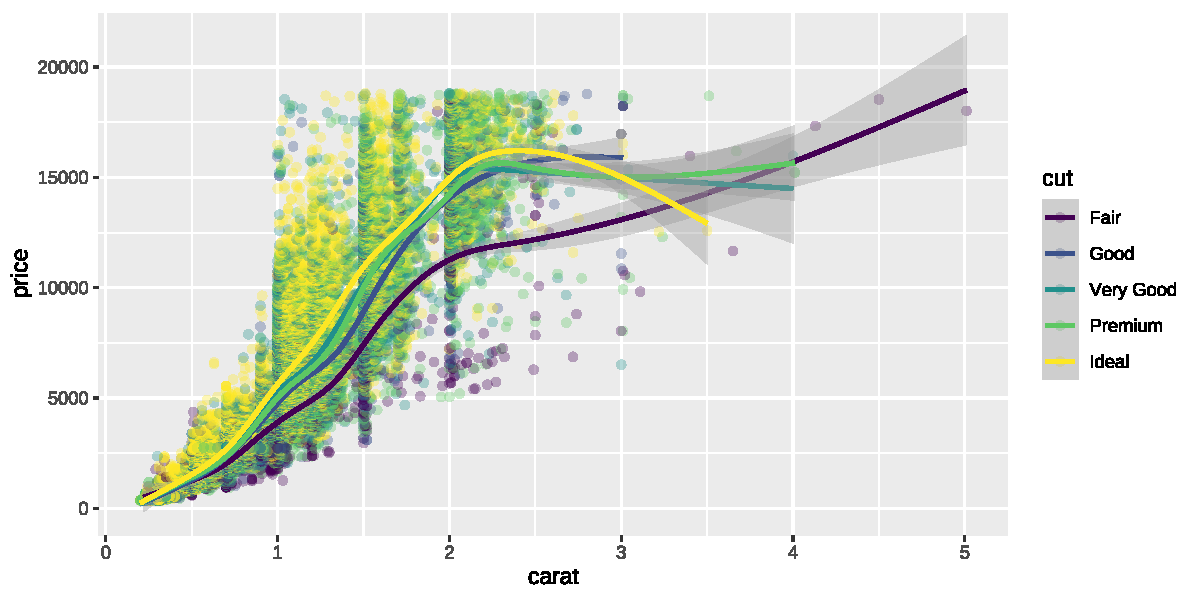
\includegraphics{2.Data_files/figure-beamer/unnamed-chunk-5-1} \end{center}
\end{frame}

\begin{frame}{课程考核}
\protect\hypertarget{ux8bfeux7a0bux8003ux6838}{}
\begin{itemize}
\tightlist
\item
  成绩评定

  \begin{itemize}
  \tightlist
  \item
    平时成绩
  \item
    考试成绩
  \end{itemize}
\item
  作业要求

  \begin{itemize}
  \tightlist
  \item
    独立思考
  \item
    演算正确
  \item
    作图清楚
  \item
    书写整齐
  \end{itemize}
\end{itemize}

\begin{center}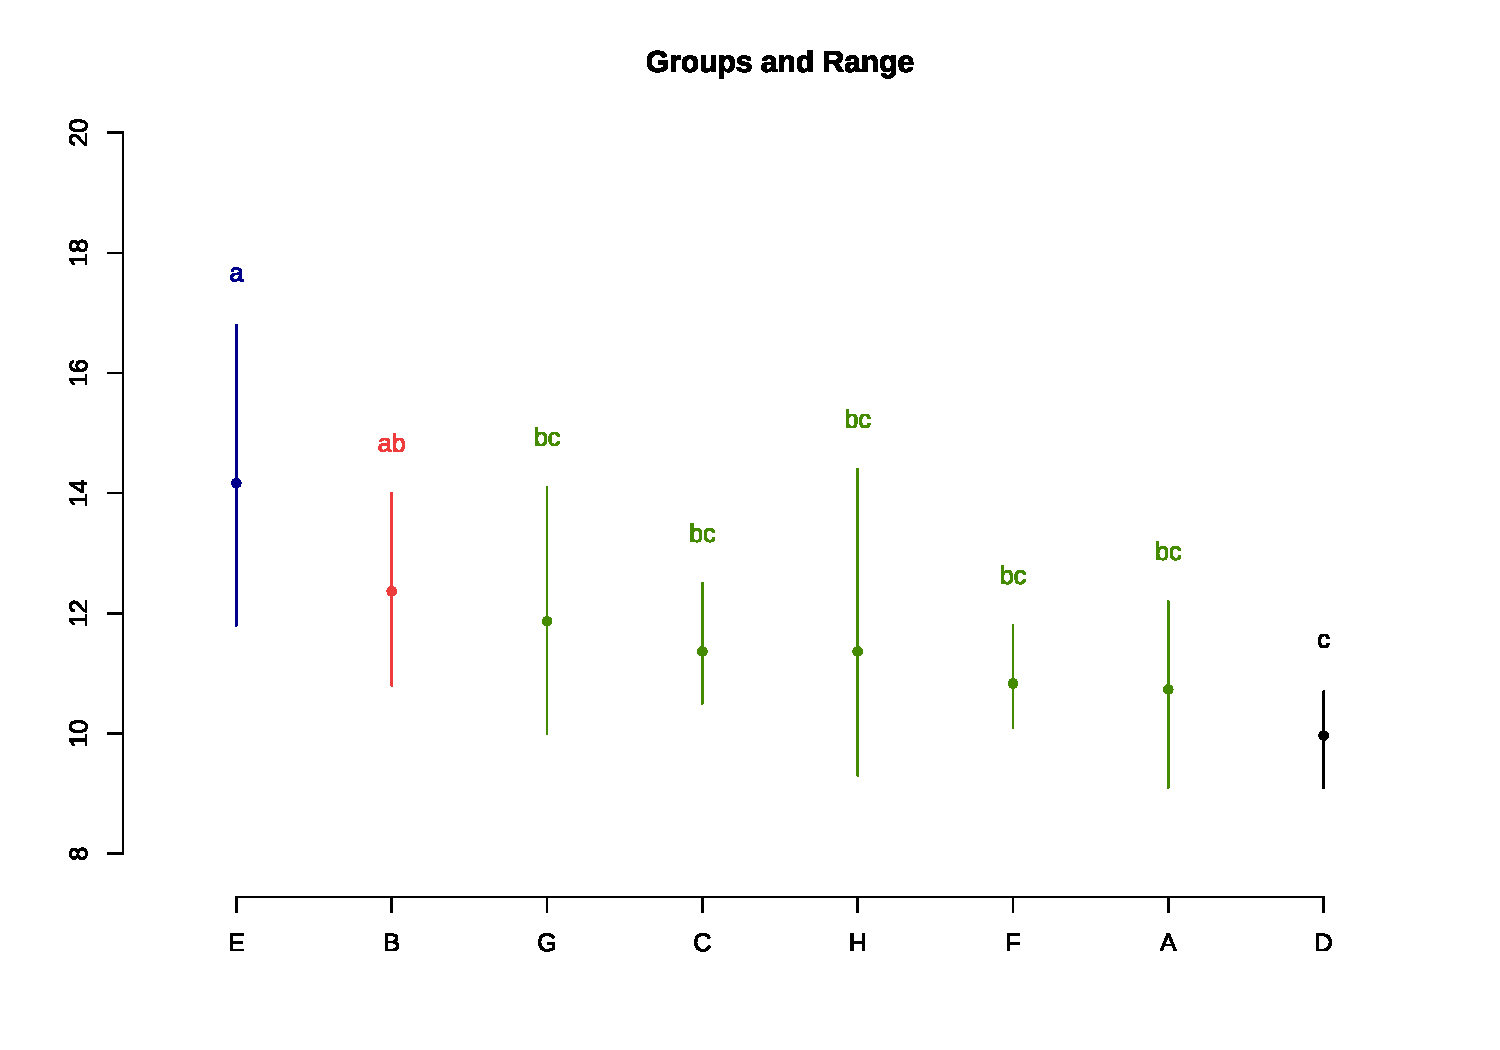
\includegraphics{2.Data_files/figure-beamer/unnamed-chunk-7-1} \end{center}
\end{frame}

\begin{frame}{学习重点}
\protect\hypertarget{ux5b66ux4e60ux91cdux70b9}{}
\begin{itemize}
\tightlist
\item
  重点讲解统计方法在生物学中的应用;
\item
  了解公式的推导和证明;
\item
  及时完成作业,按时提交和反馈。
\end{itemize}
\end{frame}

\begin{frame}{}
\protect\hypertarget{section-1}{}
\LARGE 第一章\(~\)概论
\end{frame}

\begin{frame}{第一节\(~\)生物统计学的概念}
\protect\hypertarget{ux7b2cux4e00ux8282ux751fux7269ux7edfux8ba1ux5b66ux7684ux6982ux5ff5}{}
\begin{itemize}
\item
  生物统计学是数理统计在生物学研究中的应用
\item
  用数理统计的原理和方法来分析和解释生物界各种现象和试验调查资料的科学
\item
  属于生物数学的范畴

  \begin{itemize}
  \tightlist
  \item
    涉及到数列、排列、组合、矩阵、微积分等知识
  \end{itemize}
\end{itemize}
\end{frame}

\begin{frame}{为什么要学习统计学}
\protect\hypertarget{ux4e3aux4ec0ux4e48ux8981ux5b66ux4e60ux7edfux8ba1ux5b66}{}
\end{frame}

\begin{frame}{第二节\(~\)统计学发展概况}
\protect\hypertarget{ux7b2cux4e8cux8282ux7edfux8ba1ux5b66ux53d1ux5c55ux6982ux51b5}{}
\begin{itemize}
\item
  统计实践随着计数活动开始(原始社会)
\item
  上升到理论成为系统的统计学(17世纪英国)

  \begin{itemize}
  \tightlist
  \item
    政治算数:Political Arithmetick, 1690, W. Petty.
  \item
    该书分为两部分:英法荷三国国力比较,英国国情国力和增长分析
  \end{itemize}
\item
  发展经历三个阶段

  \begin{itemize}
  \tightlist
  \item
    古典记录统计学
  \item
    近代描述统计学
  \item
    现代推断统计学
  \end{itemize}
\end{itemize}
\end{frame}

\begin{frame}{一、古典记录统计学}
\protect\hypertarget{ux4e00ux53e4ux5178ux8bb0ux5f55ux7edfux8ba1ux5b66}{}
\end{frame}

\begin{frame}{二、近代描述统计学}
\protect\hypertarget{ux4e8cux8fd1ux4ee3ux63cfux8ff0ux7edfux8ba1ux5b66}{}
\end{frame}

\begin{frame}{三、现代推断统计学}
\protect\hypertarget{ux4e09ux73b0ux4ee3ux63a8ux65adux7edfux8ba1ux5b66}{}
\end{frame}

\begin{frame}{第三节\(~\)常用统计学术语}
\protect\hypertarget{ux7b2cux4e09ux8282ux5e38ux7528ux7edfux8ba1ux5b66ux672fux8bed}{}
\begin{itemize}
\item
  总体与样本
\item
  参数与统计数
\item
  变量与资料
\item
  因素与水平
\end{itemize}
\end{frame}

\begin{frame}{一、总体与样本}
\protect\hypertarget{ux4e00ux603bux4f53ux4e0eux6837ux672c}{}
\end{frame}

\begin{frame}{二、参数与统计数}
\protect\hypertarget{ux4e8cux53c2ux6570ux4e0eux7edfux8ba1ux6570}{}
\end{frame}

\begin{frame}{三、变量与资料}
\protect\hypertarget{ux4e09ux53d8ux91cfux4e0eux8d44ux6599}{}
\end{frame}

\begin{frame}{四、因素与水平}
\protect\hypertarget{ux56dbux56e0ux7d20ux4e0eux6c34ux5e73}{}
\end{frame}

\begin{frame}{五、处理与重复}
\protect\hypertarget{ux4e94ux5904ux7406ux4e0eux91cdux590d}{}
\end{frame}

\begin{frame}{六、效应与互作}
\protect\hypertarget{ux516dux6548ux5e94ux4e0eux4e92ux4f5c}{}
\end{frame}

\begin{frame}{七、因素与水平}
\protect\hypertarget{ux4e03ux56e0ux7d20ux4e0eux6c34ux5e73}{}
\end{frame}

\begin{frame}{八、误差和错误}
\protect\hypertarget{ux516bux8befux5deeux548cux9519ux8bef}{}
\begin{itemize}
\tightlist
\item
  误差:也称为试验误差,是指观测值偏离真值的差异,分为随机误差和系统误差。

  \begin{itemize}
  \tightlist
  \item
    随机误差:由于试验中许多无法控制的偶然因素所造成的试验结果与真实值之间的差异,是\textbf{不可避免}的。
  \item
    系统误差:由于试验处理以外的其他条件明显不一致所产生的带有倾向性的或定向性的偏差。
  \end{itemize}
\item
  错误:在实验过程中,人为因素引起的差错。
\end{itemize}
\end{frame}

\begin{frame}{第四节\(~\)生物统计学的内容与作用}
\protect\hypertarget{ux7b2cux56dbux8282ux751fux7269ux7edfux8ba1ux5b66ux7684ux5185ux5bb9ux4e0eux4f5cux7528}{}
\end{frame}

\end{document}
